\documentclass[12pt]{article}

\usepackage{fontspec}
\newfontfamily\handwriting{a-casual-handwritten-pen}[Path=../assets/fonts/,Extension=.ttf,Scale=1.5]
\newfontfamily\comic{Comic Neue}

\usepackage[utf8]{inputenc}
\usepackage{amsmath}
\usepackage{amssymb}
\usepackage{enumitem}
\usepackage{xcolor}
\usepackage{soul}
\usepackage{tikz}
\usepackage[most]{tcolorbox}
\usepackage{titlesec}
\usepackage{multicol}
\usepackage{environ}

\usetikzlibrary{fit, positioning, arrows.meta, decorations.pathreplacing}

% --- Custom Colors ---
\definecolor{primaryblue}{RGB}{42, 111, 151}
\definecolor{exbg}{RGB}{255, 240, 245}
\definecolor{rulebg}{RGB}{232, 245, 233}
\definecolor{highlight}{RGB}{255, 243, 176}
\definecolor{pinkanno}{RGB}{255, 105, 180}
\definecolor{purpleanno}{RGB}{147, 112, 219}
\definecolor{solutionbg}{RGB}{245, 245, 255}

% --- Header Styling ---
\titleformat{\section}{\color{primaryblue}\normalfont\Large\bfseries}{\thesection}{1em}{}
\titleformat{\subsection}{\color{primaryblue}\normalfont\large\bfseries}{\thesubsection}{1em}{}

% --- Friendly Boxes ---
% --- Auto-numbered Example Box ---
\newcounter{examplenum}

\newtcolorbox{friendlyexbox}[1]{
    colback=exbg,
    colframe=pinkanno!50,
    arc=5pt,
    title=\textbf{#1},
    coltitle=black,
    attach title to upper,
    after title={:\quad}
}

\newenvironment{friendlyex}{%
    \refstepcounter{examplenum}%
    \begin{friendlyexbox}{Example \theexamplenum}%
}{%
    \end{friendlyexbox}%
}

\newtcolorbox{friendlyrule}[1]{
    colback=rulebg,
    colframe=primaryblue!30,
    arc=5pt,
    fonttitle=\bfseries,
    title={#1},
    coltitle=primaryblue
}

\newcommand{\funhl}[1]{\sethlcolor{highlight}\hl{#1}}

% --- Show/Hide Solutions ---
\newif\ifshowsolutions

% Uncomment the next line to show solutions.
\showsolutionstrue

\newcommand{\solutionblank}{\vspace{25ex}}

\NewEnviron{solutionbox}{
\ifshowsolutions
\begin{tcolorbox}[
    colback=solutionbg,
    colframe=purpleanno!45,
    arc=5pt,
    title={Solution},
    coltitle=primaryblue,
    fonttitle=\bfseries
]
\BODY
\end{tcolorbox}
\else
\solutionblank
\fi
}

\begin{document}
\handwriting

\begin{center}
    \Large\textbf{\color{primaryblue}Module 3 Lesson 3A\\Graphing Rational Functions} \\
    \vspace{0.2cm}
    \hrule
\end{center}

\section*{Objectives}

\begin{friendlyrule}{In this lesson, we will learn how to}
\begin{itemize}
    \item graph the toolkit functions $\dfrac{1}{x}$ and $\dfrac{1}{x^2}$;
    \item graph transformations of these toolkit functions;
    \item fully graph a rational function using domain, intercepts, asymptotes, holes, and a table of points.
\end{itemize}
\end{friendlyrule}

\section*{1. Toolkit Functions}

\begin{center}
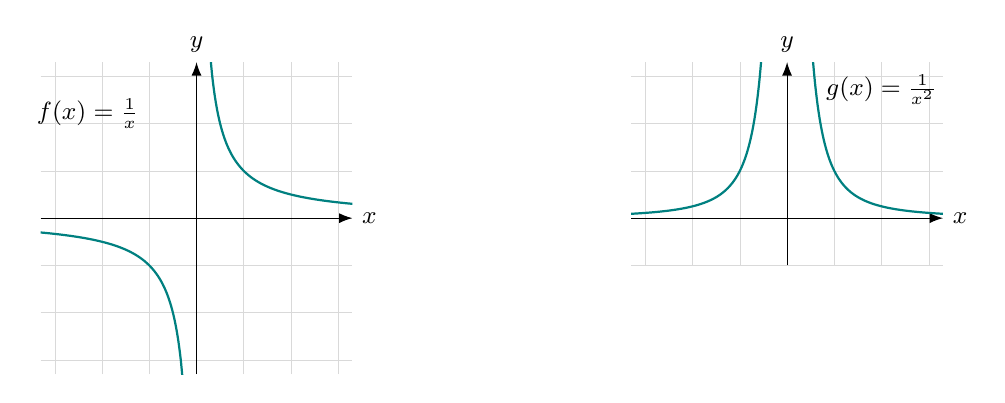
\begin{tikzpicture}
\begin{scope}[xscale=0.6,yscale=0.6]
\draw[step=1, gray!30, very thin] (-3.3,-3.3) grid (3.3,3.3);
\draw[-{Latex}] (-3.3,0) -- (3.3,0) node[right] {\small $x$};
\draw[-{Latex}] (0,-3.3) -- (0,3.3) node[above] {\small $y$};
\begin{scope}
\clip (0.28,-3.3) rectangle (3.3,3.3);
\draw[teal, thick, domain=0.28:3.3, samples=60, smooth] plot (\x, {1/\x});
\end{scope}
\begin{scope}
\clip (-3.3,-3.3) rectangle (-0.28,3.3);
\draw[teal, thick, domain=-3.3:-0.28, samples=60, smooth] plot (\x, {1/\x});
\end{scope}
\node[above] at (-2.3,1.7) {\small $f(x)=\frac1x$};
\end{scope}
\begin{scope}[xscale=0.6,yscale=0.6, shift={(12.5,0)}]
\draw[step=1, gray!30, very thin] (-3.3,-1) grid (3.3,3.3);
\draw[-{Latex}] (-3.3,0) -- (3.3,0) node[right] {\small $x$};
\draw[-{Latex}] (0,-1) -- (0,3.3) node[above] {\small $y$};
\begin{scope}
\clip (0.28,-1) rectangle (3.3,3.3);
\draw[teal, thick, domain=0.28:3.3, samples=60, smooth] plot (\x, {1/(\x*\x)});
\end{scope}
\begin{scope}
\clip (-3.3,-1) rectangle (-0.28,3.3);
\draw[teal, thick, domain=-3.3:-0.28, samples=60, smooth] plot (\x, {1/(\x*\x)});
\end{scope}
\node[above] at (2,2.2) {\small $g(x)=\frac{1}{x^2}$};
\end{scope}
\end{tikzpicture}
\end{center}

\begin{friendlyrule}{Key Features}
\begin{itemize}
    \item Both toolkit functions have a vertical asymptote at $x=0$ and horizontal asymptote $y=0$.
    \item $f(x)=\frac1x$ is an \funhl{odd} function (symmetric about the origin); its two branches lie in Quadrants I and III.
    \item $g(x)=\frac{1}{x^2}$ is an \funhl{even} function (symmetric about the $y$-axis); both branches lie above the $x$-axis, in Quadrants I and II.
\end{itemize}
\end{friendlyrule}

\section*{2. Graphing Transformations}

\begin{friendlyrule}{Transforming $\frac1x$ or $\frac{1}{x^2}$}
Writing a rational function as $\dfrac{1}{x-h}+k$ (or $\dfrac{1}{(x-h)^2}+k$) shifts the toolkit graph so that the vertical asymptote is $x=h$ and the horizontal asymptote is $y=k$.
\end{friendlyrule}

\begin{friendlyex}{}
Sketch $h(x)=\dfrac{1}{x+3}-2$.

\begin{center}
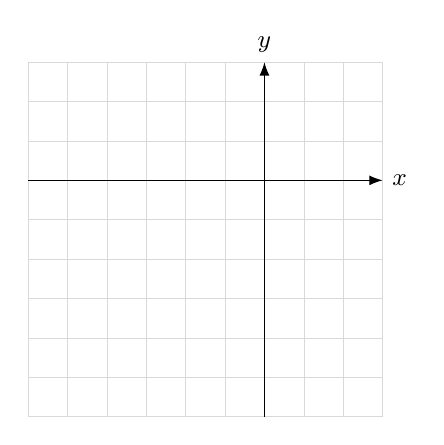
\begin{tikzpicture}[scale=0.5]
\draw[step=1, gray!30, very thin] (-6,-6) grid (3,3);
\draw[-{Latex}] (-6,0) -- (3,0) node[right] {\small $x$};
\draw[-{Latex}] (0,-6) -- (0,3) node[above] {\small $y$};
\end{tikzpicture}
\end{center}
\end{friendlyex}

\begin{solutionbox}
This is $\dfrac1x$ shifted left $3$ and down $2$. Vertical asymptote: $x=-3$. Horizontal asymptote: $y=-2$.

\begin{center}
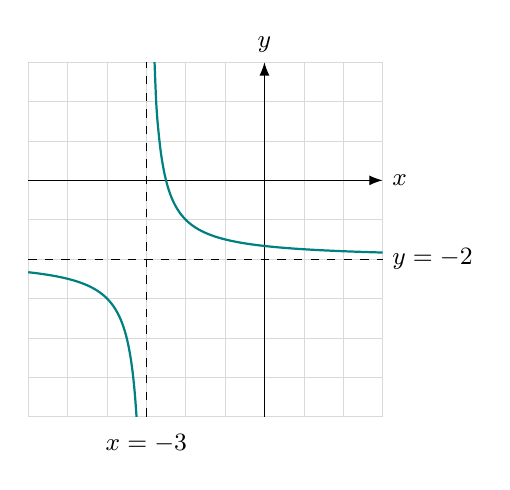
\begin{tikzpicture}[scale=0.5]
\draw[step=1, gray!30, very thin] (-6,-6) grid (3,3);
\draw[dashed] (-3,-6) -- (-3,3);
\draw[dashed] (-6,-2) -- (3,-2);
\draw[-{Latex}] (-6,0) -- (3,0) node[right] {\small $x$};
\draw[-{Latex}] (0,-6) -- (0,3) node[above] {\small $y$};
\begin{scope}
\clip (-2.85,-6) rectangle (3,3);
\draw[teal, thick, domain=-2.85:3, samples=60, smooth] plot (\x, {1/(\x+3)-2});
\end{scope}
\begin{scope}
\clip (-6,-6) rectangle (-3.15,3);
\draw[teal, thick, domain=-6:-3.15, samples=60, smooth] plot (\x, {1/(\x+3)-2});
\end{scope}
\node[below] at (-3,-6.2) {\small $x=-3$};
\node[right] at (3,-2) {\small $y=-2$};
\end{tikzpicture}
\end{center}
\end{solutionbox}

\begin{friendlyex}{}
Sketch $k(x)=-\dfrac{1}{(x-1)^2}+3$.

\begin{center}
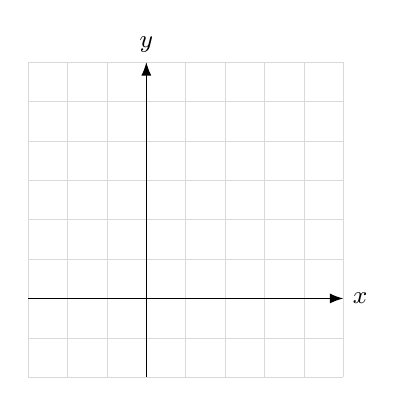
\begin{tikzpicture}[scale=0.5]
\draw[step=1, gray!30, very thin] (-3,-2) grid (5,6);
\draw[-{Latex}] (-3,0) -- (5,0) node[right] {\small $x$};
\draw[-{Latex}] (0,-2) -- (0,6) node[above] {\small $y$};
\end{tikzpicture}
\end{center}
\end{friendlyex}

\begin{solutionbox}
This is $\dfrac{1}{x^2}$ shifted right $1$, reflected over the $x$-axis, and shifted up $3$. Vertical asymptote: $x=1$. Horizontal asymptote: $y=3$.

\begin{center}
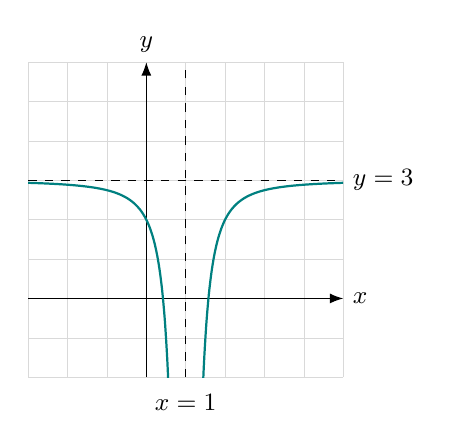
\begin{tikzpicture}[scale=0.5]
\draw[step=1, gray!30, very thin] (-3,-2) grid (5,6);
\draw[dashed] (1,-2) -- (1,6);
\draw[dashed] (-3,3) -- (5,3);
\draw[-{Latex}] (-3,0) -- (5,0) node[right] {\small $x$};
\draw[-{Latex}] (0,-2) -- (0,6) node[above] {\small $y$};
\begin{scope}
\clip (1.2,-2) rectangle (5,6);
\draw[teal, thick, domain=1.2:5, samples=60, smooth] plot (\x, {-1/((\x-1)*(\x-1))+3});
\end{scope}
\begin{scope}
\clip (-3,-2) rectangle (0.8,6);
\draw[teal, thick, domain=-3:0.8, samples=60, smooth] plot (\x, {-1/((\x-1)*(\x-1))+3});
\end{scope}
\node[below] at (1,-2.2) {\small $x=1$};
\node[right] at (5,3) {\small $y=3$};
\end{tikzpicture}
\end{center}
\end{solutionbox}

\section*{3. Reading Features from a Graph}

\begin{friendlyex}{}
Use the graph below to identify the vertical asymptote, horizontal asymptote, $x$-intercept, and $y$-intercept.

\begin{center}
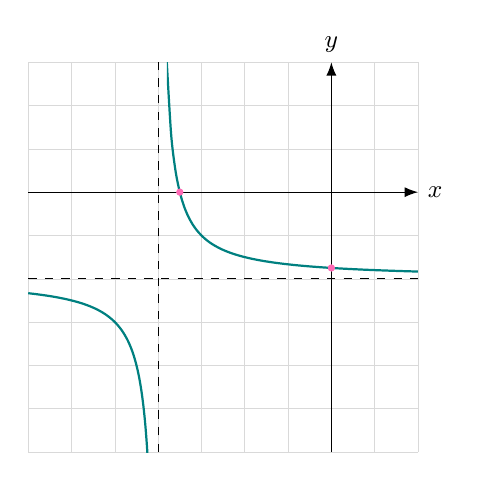
\begin{tikzpicture}[scale=0.55]
\draw[step=1, gray!30, very thin] (-7,-6) grid (2,3);
\draw[dashed] (-4,-6) -- (-4,3);
\draw[dashed] (-7,-2) -- (2,-2);
\draw[-{Latex}] (-7,0) -- (2,0) node[right] {\small $x$};
\draw[-{Latex}] (0,-6) -- (0,3) node[above] {\small $y$};
\begin{scope}
\clip (-3.8,-6) rectangle (2,3);
\draw[teal, thick, domain=-3.8:2, samples=60, smooth] plot (\x, {1/(\x+4)-2});
\end{scope}
\begin{scope}
\clip (-7,-6) rectangle (-4.2,3);
\draw[teal, thick, domain=-7:-4.2, samples=60, smooth] plot (\x, {1/(\x+4)-2});
\end{scope}
\filldraw[pinkanno] (-3.5,0) circle (2pt);
\filldraw[pinkanno] (0,-1.75) circle (2pt);
\end{tikzpicture}
\end{center}
\end{friendlyex}

\begin{solutionbox}
\textbf{Vertical asymptote:} $x=-4$. \qquad \textbf{Horizontal asymptote:} $y=-2$.

\textbf{$x$-intercept:} $(-3.5,0)$. \qquad \textbf{$y$-intercept:} $(0,-1.75)$.

(This graph matches $f(x)=\dfrac{1}{x+4}-2$: setting $f(x)=0$ gives $x=-3.5$, and $f(0)=\frac14-2=-1.75$.)
\end{solutionbox}

\section*{4. Full Worked Examples}

\begin{friendlyex}{}
Graph $f(x)=\dfrac{3}{(x+2)(x-1)}$.
\end{friendlyex}

\begin{solutionbox}
\textbf{Domain:} $x\neq -2,1$.

\textbf{Vertical asymptotes:} $x=-2,\ x=1$ (no common factors, so no holes).

\textbf{Horizontal asymptote:} numerator degree $0<$ denominator degree $2$, so $y=0$.

\textbf{$y$-intercept:} $f(0)=\dfrac{3}{(2)(-1)}=-1.5$. \qquad \textbf{$x$-intercepts:} none (numerator is never $0$).

\begin{center}
\begin{tabular}{|c|c|c|c|c|c|}
\hline
$x$ & $-4$ & $-3$ & $0.5$ & $2$ & $3$ \\
\hline
$f(x)$ & $0.3$ & $0.75$ & $-2.4$ & $0.75$ & $0.3$ \\
\hline
\end{tabular}
\end{center}

\begin{center}
\begin{tikzpicture}
\begin{scope}[xscale=0.85,yscale=0.55]
\draw[dashed, gray] (-2,-4.5) -- (-2,4.5);
\draw[dashed, gray] (1,-4.5) -- (1,4.5);
\draw[dashed, gray] (-4.3,0) -- (4.3,0);
\draw[-{Latex}] (-4.3,0) -- (4.3,0) node[right] {\small $x$};
\draw[-{Latex}] (0,-4.5) -- (0,4.5) node[above] {\small $y$};
\begin{scope}
\clip (-4.3,-4.3) rectangle (-2.08,4.3);
\draw[teal, thick, domain=-4.2:-2.08, samples=60, smooth] plot (\x, {3/((\x+2)*(\x-1))});
\end{scope}
\begin{scope}
\clip (-1.92,-4.3) rectangle (0.92,4.3);
\draw[teal, thick, domain=-1.92:0.92, samples=80, smooth] plot (\x, {3/((\x+2)*(\x-1))});
\end{scope}
\begin{scope}
\clip (1.08,-4.3) rectangle (4.3,4.3);
\draw[teal, thick, domain=1.08:4.2, samples=60, smooth] plot (\x, {3/((\x+2)*(\x-1))});
\end{scope}
\filldraw[pinkanno] (0,-1.5) circle (2pt);
\node[below] at (-2,-4.6) {\small $x=-2$};
\node[below] at (1,-4.6) {\small $x=1$};
\end{scope}
\end{tikzpicture}
\end{center}
\end{solutionbox}

\begin{friendlyex}{}
Graph $f(x)=\dfrac{x+1}{x^2+2x-3}$.
\end{friendlyex}

\begin{solutionbox}
Factor: $f(x)=\dfrac{x+1}{(x+3)(x-1)}$. The numerator shares no common factor with the denominator, so there are \textbf{no holes}.

\textbf{Domain:} $x\neq -3,1$. \qquad \textbf{Vertical asymptotes:} $x=-3,\ x=1$.

\textbf{Horizontal asymptote:} numerator degree $1<$ denominator degree $2$, so $y=0$ (and there is \textbf{no slant asymptote}, since the numerator's degree is not exactly one more than the denominator's).

\textbf{$y$-intercept:} $f(0)=\dfrac{1}{-3}=-0.33$. \qquad \textbf{$x$-intercept:} $x+1=0\implies x=-1$, i.e.\ $(-1,0)$.

\begin{center}
\begin{tabular}{|c|c|c|c|c|c|}
\hline
$x$ & $-4$ & $-2$ & $0.5$ & $2$ & $3$ \\
\hline
$f(x)$ & $0.6$ & $0.33$ & $-0.86$ & $0.6$ & $0.33$ \\
\hline
\end{tabular}
\end{center}

\begin{center}
\begin{tikzpicture}
\begin{scope}[xscale=0.7,yscale=0.9]
\draw[dashed, gray] (-3,-2.8) -- (-3,2.8);
\draw[dashed, gray] (1,-2.8) -- (1,2.8);
\draw[dashed, gray] (-5.3,0) -- (5.3,0);
\draw[-{Latex}] (-5.3,0) -- (5.3,0) node[right] {\small $x$};
\draw[-{Latex}] (0,-2.8) -- (0,2.8) node[above] {\small $y$};
\begin{scope}
\clip (-5.3,-2.7) rectangle (-3.1,2.7);
\draw[teal, thick, domain=-5.2:-3.1, samples=60, smooth] plot (\x, {(\x+1)/((\x+3)*(\x-1))});
\end{scope}
\begin{scope}
\clip (-2.9,-2.7) rectangle (0.9,2.7);
\draw[teal, thick, domain=-2.9:0.9, samples=80, smooth] plot (\x, {(\x+1)/((\x+3)*(\x-1))});
\end{scope}
\begin{scope}
\clip (1.1,-2.7) rectangle (5.3,2.7);
\draw[teal, thick, domain=1.1:5.2, samples=60, smooth] plot (\x, {(\x+1)/((\x+3)*(\x-1))});
\end{scope}
\filldraw[pinkanno] (-1,0) circle (2pt);
\filldraw[pinkanno] (0,-0.33) circle (2pt);
\node[below] at (-3,-2.9) {\small $x=-3$};
\node[below] at (1,-2.9) {\small $x=1$};
\end{scope}
\end{tikzpicture}
\end{center}
\end{solutionbox}

\begin{friendlyex}{}
Graph $f(x)=\dfrac{x^2-x-2}{x^2-4}$.
\end{friendlyex}

\begin{solutionbox}
Factor: $f(x)=\dfrac{(x-2)(x+1)}{(x-2)(x+2)}=\dfrac{x+1}{x+2}$ for $x\neq 2$.

\textbf{Hole:} at $x=2$. Hole's $y$-value: $\dfrac{2+1}{2+2}=\dfrac34=0.75$, so the hole is at $(2,0.75)$.

\textbf{Domain:} $x\neq -2,2$. \qquad \textbf{Vertical asymptote:} $x=-2$.

\textbf{Horizontal asymptote:} numerator and denominator both degree $1$ (after simplifying), ratio $\dfrac11=1$, so $y=1$.

\textbf{$y$-intercept:} $f(0)=\dfrac12=0.5$. \qquad \textbf{$x$-intercept:} $x+1=0\implies x=-1$, i.e.\ $(-1,0)$.

\begin{center}
\begin{tabular}{|c|c|c|c|c|c|}
\hline
$x$ & $-4$ & $-3$ & $-1.5$ & $1$ & $3$ \\
\hline
$f(x)$ & $1.5$ & $2$ & $-1$ & $0.67$ & $0.8$ \\
\hline
\end{tabular}
\end{center}

\begin{center}
\begin{tikzpicture}
\begin{scope}[xscale=0.6,yscale=0.55]
\draw[dashed, gray] (-2,-5.5) -- (-2,5.5);
\draw[dashed, gray] (-6.3,1) -- (6.3,1);
\draw[-{Latex}] (-6.3,0) -- (6.3,0) node[right] {\small $x$};
\draw[-{Latex}] (0,-5.5) -- (0,5.5) node[above] {\small $y$};
\begin{scope}
\clip (-6.3,-5.4) rectangle (-2.15,5.4);
\draw[teal, thick, domain=-6.2:-2.15, samples=60, smooth] plot (\x, {(\x+1)/(\x+2)});
\end{scope}
\begin{scope}
\clip (-1.85,-5.4) rectangle (6.3,5.4);
\draw[teal, thick, domain=-1.85:6.2, samples=80, smooth] plot (\x, {(\x+1)/(\x+2)});
\end{scope}
\filldraw[pinkanno] (-1,0) circle (2pt);
\filldraw[pinkanno] (0,0.5) circle (2pt);
\draw[pinkanno, thick, fill=white] (2,0.75) circle (2.2pt);
\node[below] at (-2,-5.6) {\small $x=-2$};
\node[right] at (6.3,1) {\small $y=1$};
\end{scope}
\end{tikzpicture}
\end{center}
\end{solutionbox}

\end{document}
